
\chapter{Software Version Control}
Version control (also known as revision control,
source control, or source code management) is a class of systems
responsible for managing changes to computer programs, documents,
web sites, or other collections of information. Version control is a
component of software configuration management.\\

\vspace{3mm}

A version control system serves the following purposes, among others:
\begin{enumerate}
%\item die Speicherung der Fileversionen (Revisions) mit \"Anderungskommentar,
% die Protokollierung der Änderungen, damit jederzeit nachvollzogen
% werden kann, wer wann was (warum) geändert hat.
%\item die eindeutige Kennzeichnung der Versionen und ihrer
% Abhängigkeiten (Baumstruktur),
%\item die Zugriffsregelung und (wenn möglich) automatische Abgleichung
% bei gleichzeitigen Modifikationen (Mehrbenutzerfähigkeit),
%\item Wiederherstellung bestimmter Änderungszustände/Releases
% die Gruppierung von Fileversionen zu Releases (Snapshots)
%\item
% Gleichzeitige Entwicklung mehrerer Entwicklungszweige (engl. Branches) eines
% Projektes (z.B. stabile Release-Version und  und Entwicklerversion mit
% größeren, nicht getesteten Änderungen)
\item Version control gives access to historical versions of your project.
\item You can reproduce and understand a bug report on a
past version of your software.
\item Version control enables multiple people to simultaneously
work on a single project. Each person edits his or her own copy
of the files and chooses when to share those changes with the
rest of the team.
\end{enumerate}
\ifslides
\newpage
\fi
%Es existieren zahlreiche kommerzielle und freie Softwarepakete, die sich in
%die beiden Kategorien einteilen lassen:
There are a number of available systems for version control. They all could
be divided into two categories:
\begin{description}
\item[Centralized]
In centralized version control, each user gets his or her own working
copy, but there is just one central repository. As soon as you
commit, it is possible for your co-workers to update and to see
your changes.\\
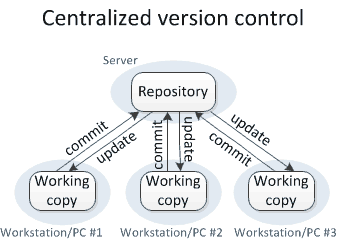
\includegraphics[width=0.5\linewidth]{config-management/version-control-fig2.png}\\
For others to see your changes, 2 things must happen:
\begin{itemize}
\item You commit
\item They update
\end{itemize}

%Diese Systeme zeichnen sich durch eine zentrales
%  Archiv (Repository) aus, wo die Originaldateien abgelegt sind. Beispiele sind:
Typical systems are:
  \begin{itemize}
  \item CVS
  \item Subversion
  \end{itemize}

\item[Distributed]
In distributed version control, each user gets his or her own
repository and working copy. After you commit, others have no access
to your changes until you push your changes to the central repository.
A pull needs to be executed to get new data into your local repository.\\
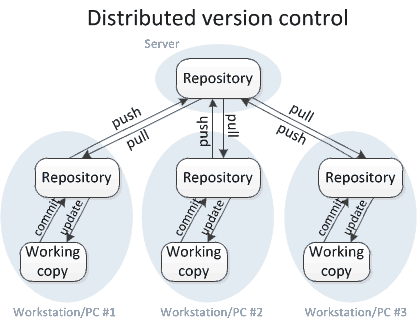
\includegraphics[width=0.5\linewidth]{config-management/version-control-fig3.png}\\
For others to see your changes, 3 things must happen:
\begin{itemize}
\item You commit
\item You push
\item They pull/fetch
\end{itemize}
  %bei diesen Systemen sind die Dateien lokal auf den
  %jeweiligen Entwicklungssystemen abgelegt (Distributed Version
  %Control System DVCS). Beispiele sind:
Typical systems are:
  \begin{itemize}
  \item GNU Arch
  \item Bazaar-NG
  \item BitKeeper
  \item Git
  \item Monotone
  \item Mercurial
  \end{itemize}
\end{description}
\ifslides
\newpage
\fi

There is also another way to classify version control systems:

\begin{description}
\item[Lock-Modify-Unlock] (Pessimistic Revision Control)\\
Many version control systems use a lock-modify-unlock model to
address the problem of many authors clobbering each other's work.
In this model, the repository allows only one person to change a
file at a time. This exclusivity policy is managed using locks.
%Einzelne Dateien müssen vor einer
%  Än\-derung gesperrt und nach Abschluss der Änderung wieder freigegeben werden.
\item[Copy-Modify-Merge] (Optimistic Revision Control)\\
Other version control systems use a copy-modify-merge model as an
alternative to locking. In this model, each user's client contacts the
project repository and creates a personal working copy. This is a local
reflection of the repository's files and directories.
Users then work simultaneously and independently, modifying their
private copies. Finally, the private copies are merged together into a
new, final version. The version control system often assists with
the merging, but ultimately a human being is responsible for making it
happen correctly.
%   Die Dateien können von allen Benutzern
%  geändert werden. Gleichzeitig durchgeführte Änderungen werden anschliessend
%  entweder automatisch oder manuell zusammengeführt.
\end{description}
%%% End:
\newslide
\newpage
\section{Git}
Git is software for tracking changes in any set of files,
usually used for coordinating work among programmers collaboratively
developing source code during software development. Its goals include
speed, data integrity, and support for distributed, non-linear workflows
(several branches running on different systems).\\

Git was created by Linus Torvalds in 2005 for development of the
Linux kernel, with other kernel developers contributing to its initial
development. Since 2005, Junio Hamano has been the core maintainer.
As with most other distributed version control systems, and unlike most
client–server systems, every Git directory on every computer is a
full-fledged repository with complete history and full version-tracking
abilities, independent of network access or a central server.
Git is free and open-source software

%GIT\footnote{englischer Slangausdruck: Blödmann, Depp}
% ist ein einfaches, von Linus Torvalds 2005 für das
% Linux-Kernel-Projekt
%in wenigen Monaten entwickeltes
%Versionsverwaltungssystem. Torvalds nennt es ein ``stupid
%(but extremely fast) directory content manager''. Anstoss dazu gab eine
%längere Auseinandersetzung mit dem Hersteller von BitKeeper, dem bis anhin von
%den Kernel-Entwicklern eingesetzten
%Versionsverwaltungssystems. Hauptkritikpunkt
%an CVS und anderen quell-offenen Paketen waren Performance-Probleme, die bei
%der grossen Anzahl von Dateien (mehr als 30 000) und der hohen Änderungsrate
%auftraten: ``Taking tens of seconds to apply a patch just because the source
%base is big is just not acceptable''. Mittlerweile geniesst Git (nebst
%Mercurial) eine grosse Popularität und wird in einer wachsenden Zahl von
%kleinen bis hin zu sehr grossen Projekten eingesetzt.

\newslide
The most important features are:
\begin{itemize}
\item \structure{Distributed repositories}:\\
each user gets his or her own repository and working copy.
\item \structure{Branches and tags}:\\
Branches and tags are part of the repository (compared to centralized systems)
\item \structure{Revision identifier}:\\
The SHA1 of the commit is the hash of all the information.
\item \structure{Commits are snapshots}:\\
In other version control systems, changes to individual files are tracked
and referred to as revisions, but with git you are tracking the entire
workspace, so they use the term snapshot to denote the difference.
\item \structure{Stages}: Files have one of the following stages: untracked,
  modified, staged, committed
\end{itemize}

%\begin{itemize}
%
% http://wiki.phys.ethz.ch/readme/git_basics
%\item Single Repository Coupled with the Project
%\item Synchronizing Production and Developer Copies
%\item Bare repository
%\end{itemize}

%
%Eigenschaften;
%\begin{itemize}
%\item Git ist eher ein Dateisystem als eine klassische Versionsverwaltung.
%\item Fast alle Operationen sind lokal
%\end{itemize}

%Git unterscheidet 4 Objekt-Typen:
\subsection{Git Object Store}
The object store contains the original data files and all the log
messages, author information, dates, and other information required to
rebuild any revision or branch of the project.\\
There are 4 different object types:
\begin{itemize}
\item \structure{Blob}: A blob is used to store file data. It is generally a file.
\item \structure{Tree}: A tree is basically like a directory.
It references a bunch of other trees and blobs
\item \structure{Commit}: A commit object holds metadata for each change
introduced in the repository, including the author, committer, commit-data,
and log messages.
\item \structure{Tag}: A tag object assigns an arbitrary human-readable
name to a specific object usually a commit.
\end{itemize}
%\ifslides
%\else
%\newpage
%\fi
All Git objects have a 160 bit hash key:
\begin{lstlisting}
6ff87c4664981e4397625791c8ea3bbb5f2279a3
\end{lstlisting}
There is a very high probability, that Git objects are globally unique.\\

\vspace{3mm}

\newslide
Git objects are stored in the \verb|.git| directory. They are reflecting a
directed acyclic graph:
\ifslides
\begin{center}
  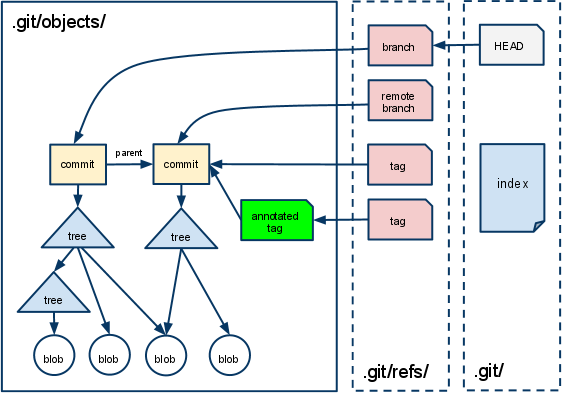
\includegraphics[width=0.7\linewidth]{config-management/git-objects}
\end{center}
\else
\begin{figure}[H]
  \centering
  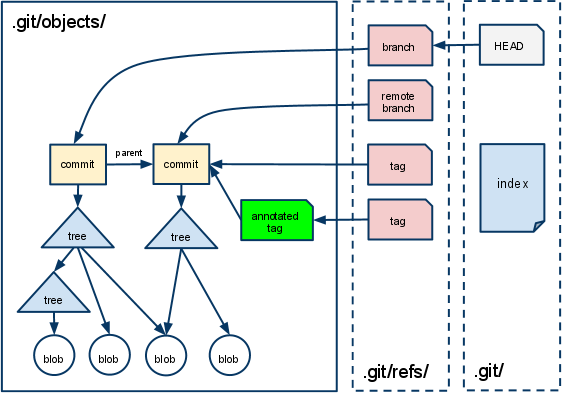
\includegraphics[width=0.7\linewidth]{config-management/git-objects}
  \caption[Git-Objekte und Referenzen]{Git objects and references \\
(Source: \href{http://teohm.github.com/blog/2011/05/30/learning-git-internals-by-example}
                {teohm.github.com/blog/2011/05/30/learning-git-internals-by-example})}
  \label{fig:gitobjects}
\end{figure}
\fi
\newslide
One of the biggest advantages of Git compared to other systems is the easy
handling of branches. Branches are needed for:
\begin{itemize}
\item executing experiments
\item try out new ideas
\item development of new features
\end{itemize}
Or in general, for any type of modification.\\
In some software projects, it is forbidden to push directly to the master
branch. Therefore it is needed to create a branch for each modification.
%
\newslide
\newpage
\subsection{Git commands}
\ifslides
\begin{center}
  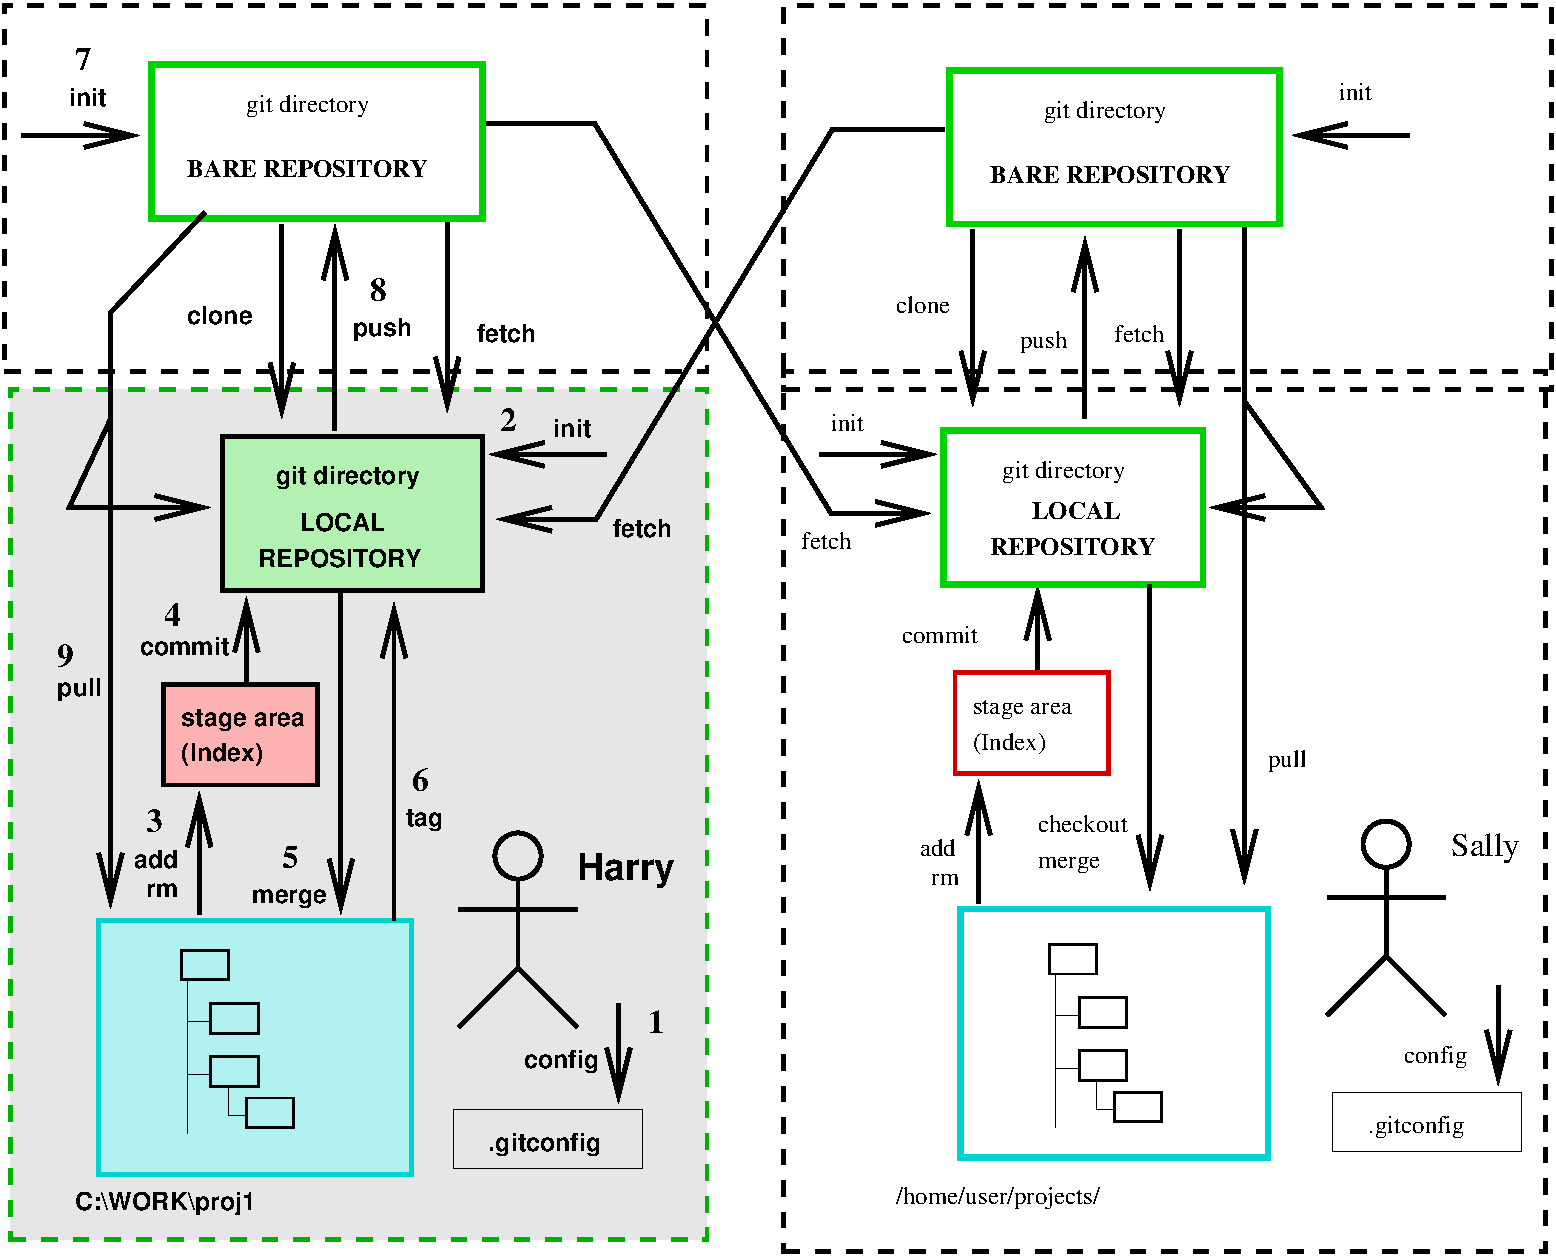
\includegraphics[width=0.65\linewidth]{config-management/xfig/git-workflow}
\end{center}
\else
\begin{figure}[H]
\centering
  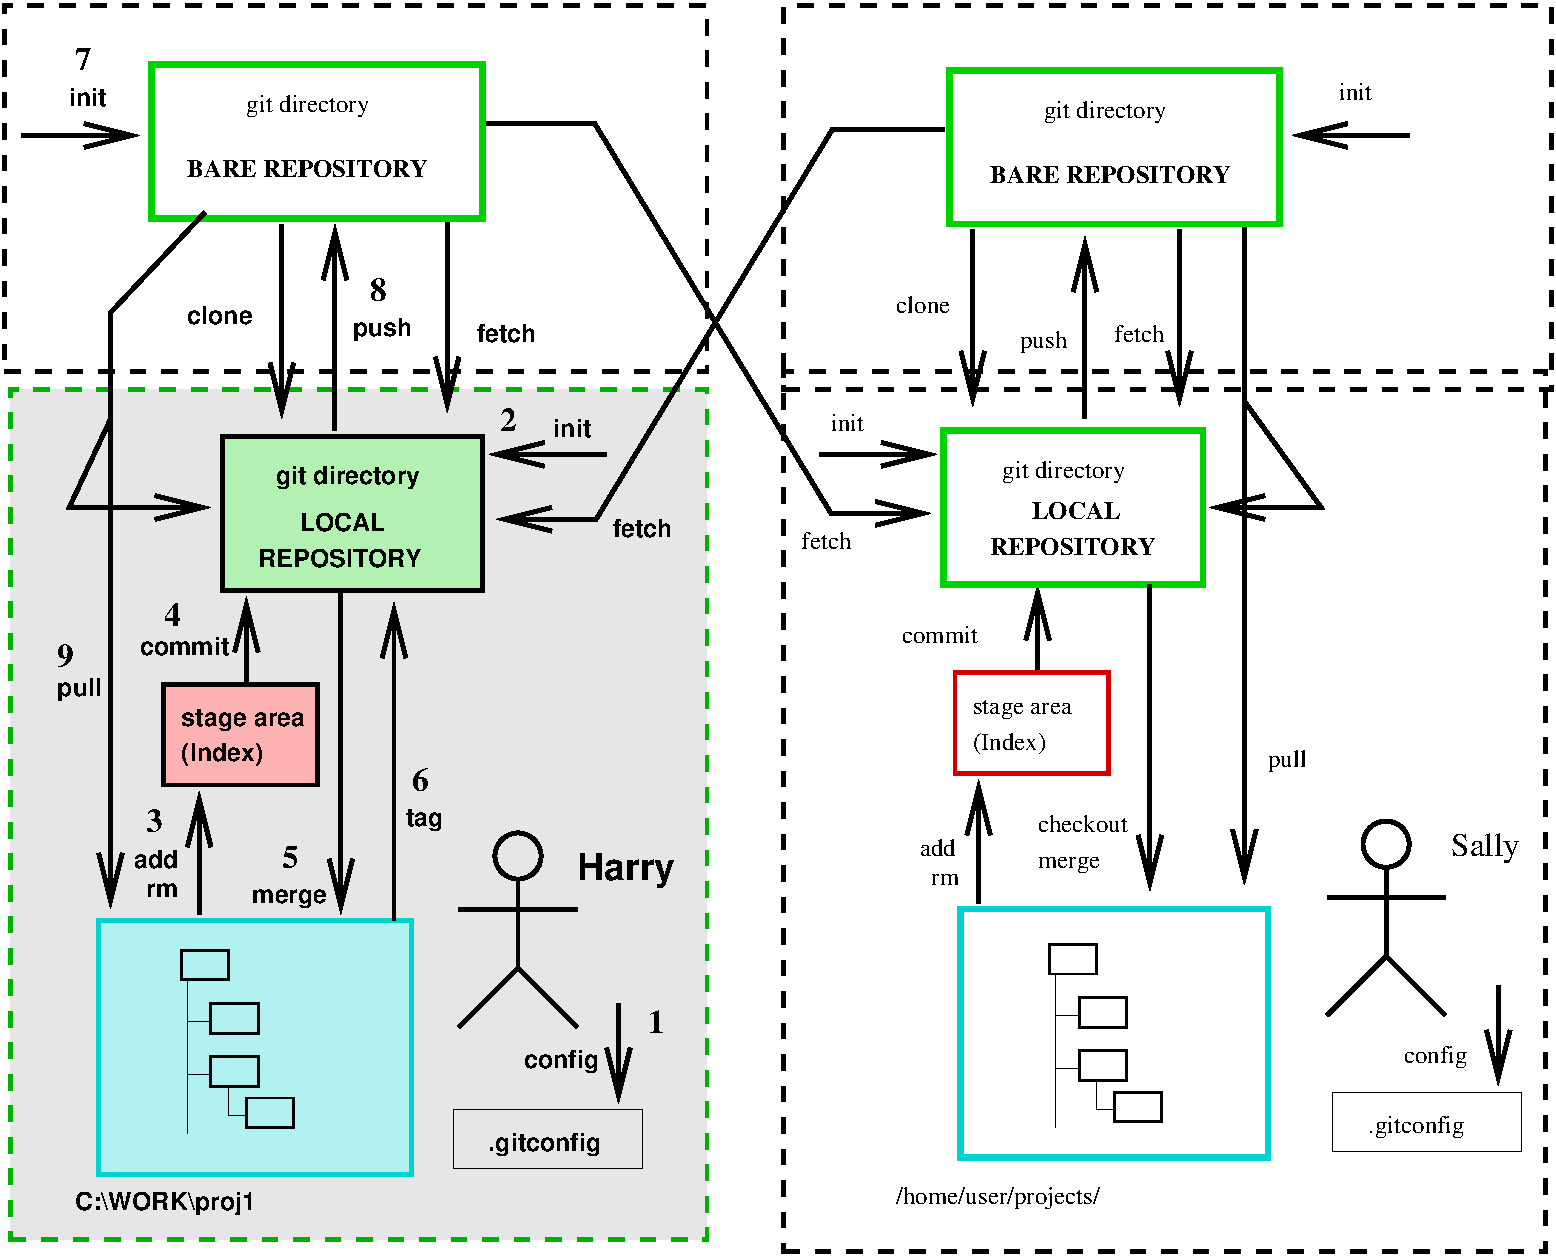
\includegraphics[width=0.95\linewidth]{config-management/xfig/git-workflow}
\caption{Workflow with git}
\end{figure}
\fi
\begin{enumerate}
\item \underline{config}: Define user name and mail address:
  \begin{lstlisting}
$ git config --global user.name "David Herzig"
$ git config --global user.email "dave.herzig@gmail.com"
  \end{lstlisting}
This information will be stored in the home directory in a file called
\verb+.gitconfig+.

There are 3 locations/levels for config files:
\begin{itemize}
\item User level
\item Repository level
\item System level
\end{itemize}

If you remove the \verb|--global| switch, the configuration will be
stored in the current repository.

%Es gibt 3 Orte für
%Config-Dateien: per User, per Repository, per System. Lässt man
%die
%Option \verb+--global+ weg, dann wird die Einstellung in der
%Config-Datei des aktuellen Repository's abgelegt.
%
\newslide
\item \underline{init}:
  create a new repository.
%  ein neues Repository einrichten. Man
%  unterscheidet lokale (private) und synchronisierbare (shared)
%  Repositories, die anderen Benutzer zugänglich gemacht werden können.

Create an empty local repository in the current directory:
  \begin{lstlisting}
$ cd /home/user/projects
$ git init project1
Initialized empty Git repository in /home/user/projects/project1/.git
  \end{lstlisting}
\begin{center}
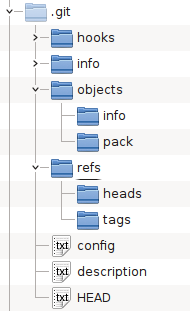
\includegraphics[width=0.25\linewidth]{config-management/git-repository-files}
\end{center}
%
{\bfseries Note:} To create a local repository from an existing one,
the command \verb|init| needs to be replaced with \verb|clone|.

%Um ein lokales Repository aus einem bereits existierenden
%zu erzeugen, muss anstelle von ``init'' der Befehl ``clone'' verwendet
%werden:

\begin{lstlisting}
$ git clone file:///var/git/project1.git
\end{lstlisting}
%
\newslide
\item \underline{add}: Adds files in the to the staging area for Git.
  \begin{lstlisting}
$ cd project1
$ git add .
  \end{lstlisting}
%$
All files in the current directory and sub directories will be added.
%Alle im aktuellen Verzeichnis liegenden Dateien und Unterverzeichnisse
%werden in die Versionsverwaltung aufgenommen (genauer: dem
%Stage-Bereich, resp. dem Index hinzugefügt)
%%% git config --global http:sslVerify false
%% env GIT_SSL_NO_VERIFY=true git clone ....
%
\newslide
\begin{center}
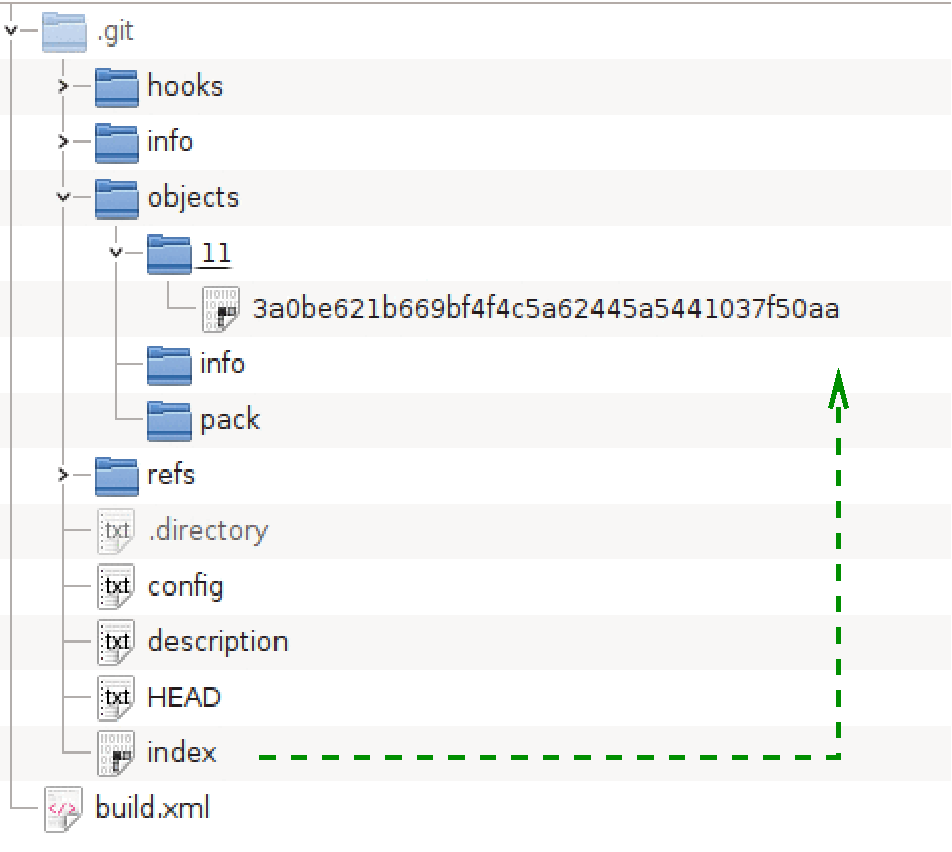
\includegraphics[width=0.7\linewidth]{config-management/xfig/git-added}
\end{center}
%% show index
%% git ls-files --stage
%%
%%%Inhalt anzeigen: git show d2ad210a...
%% 1. cat .git/HEAD:
%%    refs/heads/master
%% 2. cat .git/refs/heads/master
%%    f0dda106c105f9b15b379678d8d88322da5abd2d
%% 3. git cat-file -p f0dda106c105f9b15b379678d8d88322da5abd2d
%%    tree e4978d4515571fce768e1bb11b492e42faae7389
%%    author Ronald Tanner <tar@semafor.ch> 1410001976 +0200
%%    committer Ronald Tanner <tar@semafor.ch> 1410001976 +0200
%%
%%    initial commit
%% 4. git cat-file -p e4978d4515571fce768e1bb11b492e42faae7389
%%    100644 blob 113a0be621b669bf4f4c5a62445a5441037f50aa    build.xml
%%
%% ----------------
%% keep password
%% git config --global credential.helper cache
%%
\newslide
\item \underline{commit}: Record the changes made to the files to a local repository. For easy reference, each commit has a unique ID:
  \begin{lstlisting}
$ git commit -m "initial commit"
  \end{lstlisting}
%$
{\bfseries Note}:
  modified files needs to be added with the \verb|add| command.
  Use the option \verb|-u| to add all modified files.
  %modifizierte Dateien müssen vorgängig mit ``add'' in den
  %Stage-Bereich kopiert werden, wenn sie in das Repository übertragen
  %werden sollen. Will man alle modifizierten Dateien übertragen, kann
  %man auch die Option ``-a'' angeben:
  \begin{lstlisting}
$ git commit -am "another commit"
  \end{lstlisting}
%%% $
\begin{center}
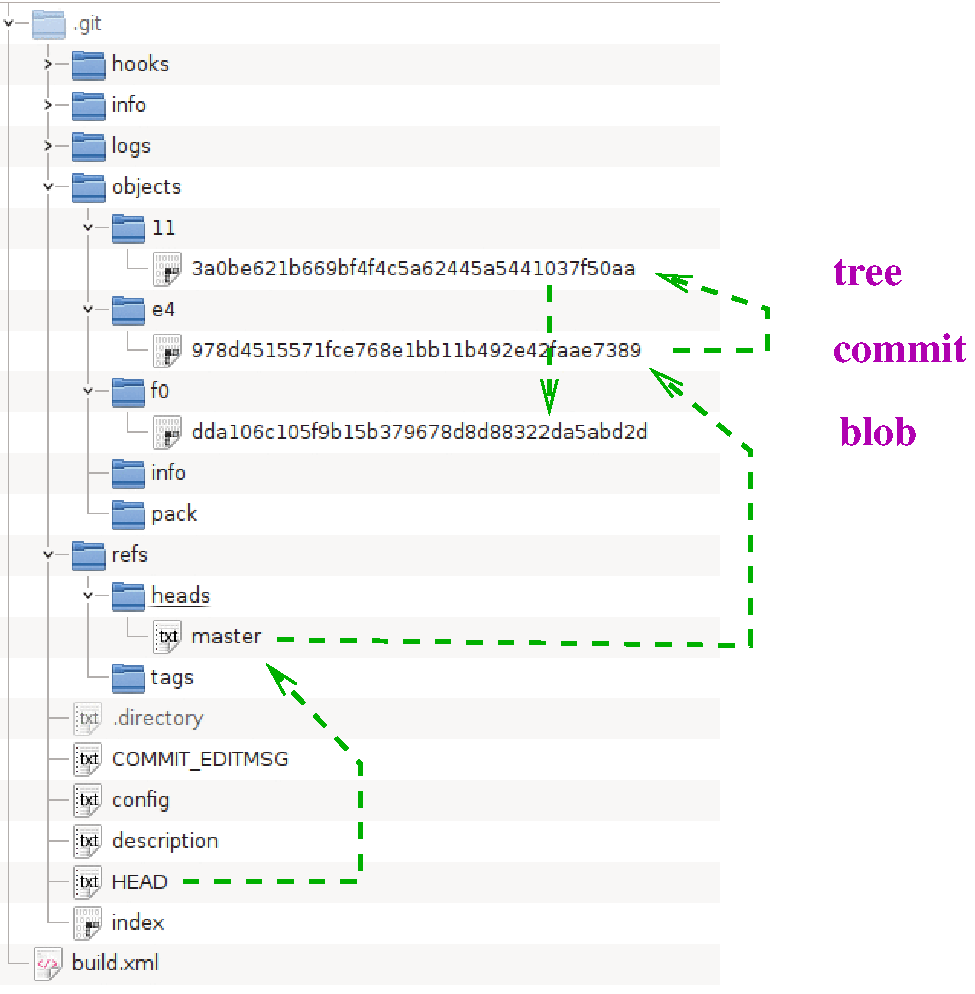
\includegraphics[width=0.66\linewidth]{config-management/xfig/git-commited}
\end{center}
\newslide
\item \underline{checkout}: To start working in a different branch, use git checkout to switch branches.
%Üblicherweise wird dazu ein neuer Branch erstellt:
  \begin{lstlisting}
$ git checkout -b ticket-53
  \end{lstlisting}
%$
\newslide
\item \underline{tag}: Git has the ability to tag specific points in a repository’s history as being important. Typically, people use this functionality to mark release points:
\begin{lstlisting}
$ git tag -a rel-0.0 -m "Release 0.0"
\end{lstlisting}
%$
{\bfseries Note}:
Git supports two types of tags: lightweight and annotated.\\
A lightweight tag is very much like a branch that doesn’t change.
It’s just a pointer to a specific commit.\\
Annotated tags, however, are stored as full objects in the Git database.
They’re checksummed; contain the tagger name, email, and date;
have a tagging message; and can be signed and verified with GNU
Privacy Guard (GPG). It’s generally recommended that you create
annotated tags so you can have all this information; but if you want
a temporary tag or for some reason don’t want to keep the other
information, lightweight tags are available too.

%Man unterscheidet lighweight und annotated
%Tags. Lightweight Tags werden ohne die Option \verb+-a+ (und ohne
%Kommentar) erstellt. Sie sind lediglich eine Referenz zu einem
%speziellen Commit. Annoted Tags werden als Objekte im Repository
%gespeichert und sind die bevorzugte Variante.

Display all tags:
\begin{lstlisting}
$ git tag -l
\end{lstlisting}
%$
\newslide
\item \underline{init}:
This command turns a directory into an empty Git repository. This is the first step in creating a repository. After running git init, adding and committing files/directories is possible.
\begin{lstlisting}
$ git init --bare /var/git/project1.git
\end{lstlisting}
%$

\newslide
\item \underline{push}: Sends local commits to the remote repository. git push requires two parameters: the remote repository and the branch that the push is for.
  \begin{lstlisting}
$ git remote add origin file:///var/git/project1
$ git push origin master
  \end{lstlisting}
{\bfseries Note}:
\begin{itemize}
\item User needs write permission on the repository.
\item With ``remote add'' an alias for a remote repository will be generated (in this case origin)
\item Display all remote repositories URL:
  \begin{lstlisting}
$ git remote -v
  \end{lstlisting}
%$
\item Tags are not automatically transferred to the remote repository. This
needs to be done in addtion:
%\item Tags werden nicht automatisch aus dem lokalen Repository
%  übertragen. Sie müssen explizit angegeben werden:
  \begin{lstlisting}
$ git push origin rel-0.0
  \end{lstlisting}
%$
or all together:
\begin{lstlisting}
$ git push origin --tags
\end{lstlisting}
\end{itemize}
%
\item \underline{pull}: To get the latest version of a repository run git pull. This pulls the changes from the remote repository to the local computer.
  \begin{lstlisting}
$ git pull
\end{lstlisting}
\end{enumerate}
%$
{\bfseries Note}:
the default repository and default branch could/should be defined in the
Git configuration file.
%in der Git-Config-Datei sollte/kann das Default-Repository
%und der Default-Branch definiert werden:
  \begin{lstlisting}
git config branch.master.remote origin
git config branch.master.merge refs/heads/master
  \end{lstlisting}
These values are automatically set after a \verb|git clone| operation.
%Nach einer Git-Clone-Operation sind diese Werte automatisch gesetzt.
%
\subsection{Additional operations}
\begin{itemize}
\item Get a specific version:
  \begin{lstlisting}
$ git checkout -b branch-0 rel-0.0
  \end{lstlisting}
%$
\item Display changes of a file:
\begin{lstlisting}
$ git log Main.java
\end{lstlisting}
%$
\item Detailed display of the last 2 changes of a file:
%\item Detaillierte Anzeige der letzten beiden Änderungen einer Datei:
\begin{lstlisting}
$ git log -p -2 Main.java
\end{lstlisting}
%$
\item Detailed display of the changes in the last 2 weeks:
%\item Detaillierte Anzeige Änderungen der letzten beiden Wochen:
\begin{lstlisting}
$ git log --sinde=2.weeks
\end{lstlisting}
%$
\item Display changes of a file in the stage area:
%\item Vergleich der Änderungen einer Datei mit Stage-Bereich:
\begin{lstlisting}
$ git diff Main.java
\end{lstlisting}
%$
\item Compare stage area and repository:
\begin{lstlisting}
$ git diff --staged
\end{lstlisting}
%$
\item Remove files:
\begin{lstlisting}
$ git rm Main.java
\end{lstlisting}
The file will be marked as deleted after the commit.
%Die Datei wird nach einem Commit im Repository als gelöscht markiert.
% $
\item rename a file:
\begin{lstlisting}
$ git mv Main.java NewMain.java
\end{lstlisting}
The changes will transferred into the repository after the commit.
%Die Änderung wird nach einem Commit in das Repository übertragen.
%$
\item display current state
\begin{lstlisting}
$ git status
\end{lstlisting}
\end{itemize}
%$
\subsection{Branches}
A branch in Git is simply a lightweight movable pointer to one of these
commits. The default branch name in Git is master. As you start making
commits, you’re given a master branch that points to the last commit you
made. Every time you commit, the master branch pointer moves forward
automatically.\\
Changes are normally done on a branch. After the change is completed, the
branch will be merged back into the master branch.
%Änderungen werden bei Git in der Regel nicht direkt auf dem
%Master-Branch sondern in einem separaten Branch durchgeführt, der
%(in der Regel)
%nach Abschluss der Änderungen mit dem Master-Branch zusammengeführt und
%anschliessend gelöscht wird:
\begin{itemize}
\item Create new branch:
\begin{lstlisting}
$ git checkout -b ticket-53
\end{lstlisting}
%$
\item Display all branches:
  \begin{lstlisting}
$ git branch
  \end{lstlisting}
{\bfseries Note}: remote branches will be displayed by using the option
\verb|-a|
%$
\item Commit changes:
  \begin{lstlisting}
$ git commit -m "initial commit"
  \end{lstlisting}
%$
\item Change and merge branch
  \begin{lstlisting}
$ git checkout master
$ git merge ticket-53
  \end{lstlisting}
  If there are no conflicts, the changes will be transferred into the
  repository.
%Wenn dabei keine Konflikte auftreten, werden die Änderungen
%automatisch in das Repository übertragen.
\item Delete branch
  \begin{lstlisting}
$ git branch -d ticket-53
  \end{lstlisting}
%$
\end{itemize}
%
\newslide
\subsection{Conflicts}
A conflict could occur if 2 or more developers work on the same file(s).
%Wenn 2 oder mehr Entwickler ihre Änderungen in ein gemeinsames
%Remote-Repository übertragen, oder 2 oder mehr Branches zusammengefügt
%werden, kann es zu Konflikten kommen.

Example:
\begin{lstlisting}[escapechar=\%]
$ %{\bfseries git push origin master}%
To file:///var/git/project1.git
 ! [rejected]        master -> master (non-fast-forward)
error: failed to push some refs to 'file:///var/git/project1.git'
To prevent you from losing history, non-fast-forward updates were rejected
Merge the remote changes (e.g. 'git pull') before pushing again.  See the
'Note about fast-forwards' section of 'git push --help' for details.
\end{lstlisting}
%$
\newslide
After a \verb|git pull| the following messages could be displayed:
%Nach einem Git-Pull können folgende Meldungen angezeigt werden:
\begin{lstlisting}
Auto-merging <filename>
CONFLICT (content): Merge conflict in <filename>
Automatic merge failed; fix conflicts and then commit the result
\end{lstlisting}
The lines with conflicts will be marked in the file:
%Die Konfliktstellen der betreffenden Dateien sind
%ähnlich wie bei Subversion markiert mit den Zeilen
\begin{lstlisting}
<<<<<<<
=======
>>>>>>>
\end{lstlisting}
These conflicts needs to be fixed manually.
%Diese Stellen müssen korrigiert werden, bevor man die Änderungen per
%commit übertragen kann.
% Bei
% der Bezeichnung project1.git handelt es sich eine Namenskonvention.
%
% http://www.thomas-krenn.com/de/wiki/Git_Workflows
\newslide

%
%http://www.kernel.org/pub/software/scm/git/docs/everyday.html
%
% self signed certs:
%% get certificate
% openssl s_client -connect host:port -key our_private_key.pem -showcerts -cert our_server-signed_cert.pem
%
% save it in /etc/ssl/certs
%
%% clone:
% GIT_SSL_CAINFO=/etc/ssl/certs/rorcz_root_cert.pem \
%    git clone https://repo.or.cz/org-mode.git
%
%# Ensure all future interactions with origin remote also work
% cd org-mode
% git config http.sslCAInfo /etc/ssl/certs/rorcz_root_cert.pem

%
\newslide
\section{Exercise}
\begin{enumerate}
\item Perform the following steps on the data loader component:
\begin{itemize}
\item Create a repository (e.g. Github, Gitlab)
\item Push your code into that repository
\item Think about the following questions:\\
Which parts of the project should be in the repository?
Which parts of the project should NOT be in the repository?
\item Create a tag which marks the software with \verb|V0_1|
\item Verify in the web console (Github, Gitlab) if
everything is correct.
\item Create a branch and perform a modification on that branch.
\item Merge the branch into the master branch.
\end{itemize}

\end{enumerate}
%{\bfseries Bewertung:} Vollständigkeit, Korrektheit, Nachvollziehbarkeit
%, Anschaulichkeit
% patch -p0 -i ~/milestone2.patch
% patch -p0 -i ~/milestone3.patch
\newslide

\section{Software and further Informations}
\begin{itemize}
\item Git project: \href{http://git-scm.com/}{git-scm.com}
\item Git tutorials: \href{http://www.gitguys.com}{www.gitguys.com},
   \href{https://www.atlassian.com/git/tutorials}{www.atlassian.com/git/tutorials}
\item 8 ways to share your git repository (Patrick Debois):\\
  \href{http://agile.dzone.com/news/8-ways-share-your-git}
   {}http://agile.dzone.com/news/8-ways-share-your-git
\item Git Workflows \href{https://www.atlassian.com/git/workflows}
         {www.atlassian.com/git/workflows}
\item Pro Git (Benutzeranleitung)
  \href{http://progit.org/book}{progit.org/book}
\item Git Reference: \href{http://gitref.org}{gitref.org}
\item Git -- Verteilte Versionsverwaltung für Code und Dokumente,
(V. Haenel, J. Plenz, Open Source Press, 2011)
\href{http://gitbu.ch}{gitbu.ch}
\item Eclipse-Plugin EGit:
  \href{http://www.eclipse.org/egit}{www.eclipse.org/egit}
\item TortoiseGit: \href{http://code.google.com/p/tortoisegit}
    {code.google.com/p/tortoisegit}
\item Configuration management with Subversion,
  Ant and Maven (Gunther Popp) dpunkt.verlag, 2008
\label{lit:popp}
%\item CVS
%\begin{itemize}
%\item CVS Project:
%  \href{http://savannah.nongnu.org/projects/cvs/}
%    {savannah.nongnu.org/projects/cvs/}
%\item Open Source Development with CVS:
%  \href{http://cvsbook.red-bean.com}{cvsbook.red-bean.com}
%\item CVS Client/Server für Windows 2000/XP:
%  \href{http://www.march-hare.com/cvspro}{www.march-hare.com/cvspro}
%\item Ein CVS-Client-Front-End für MS-Explorer:
%  \href{http://www.tortoisecvs.org}{www.tortoisecvs.org}
%\item Mehrere graphische Frontends für CVS:
%  \href{http://www.wincvs.org}{www.wincvs.org}
%\end{itemize}
\item Additional versioning tools:
\begin{itemize}
\item Mercurial: \href{http://mercurial.selenic.com/}{mercurial.selenic.com}
\item Monotone:
  \href{http://www.monotone.ca}{www.monotone.ca}
\item GNU arch:
  \href{http://www.gnu.org/s/gnu-arch}{www.gnu.org/s/gnu-arch}
\end{itemize}
\end{itemize}
%---------------------------------------------------------------

%%% Local Variables:
%%% mode: latex
%%% TeX-master: t
%%% End:
